\section{eo\-St\-Point\-Mutation$<$ FType, Node $>$ Class Template Reference}
\label{classeo_st_point_mutation}\index{eoStPointMutation@{eoStPointMutation}}
eo\-St\-Point\-Mutation --$>$ replace a Node with a Node of the same arity and type  


{\tt \#include $<$gp/eo\-St\-Parse\-Tree\-Op.h$>$}

Inheritance diagram for eo\-St\-Point\-Mutation$<$ FType, Node $>$::\begin{figure}[H]
\begin{center}
\leavevmode
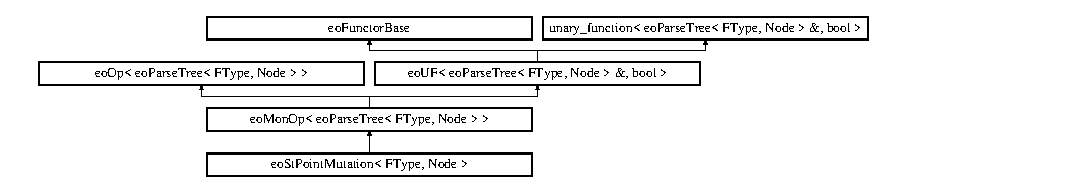
\includegraphics[height=2.14559cm]{classeo_st_point_mutation}
\end{center}
\end{figure}
\subsection*{Public Types}
\begin{CompactItemize}
\item 
typedef {\bf eo\-Parse\-Tree}$<$ FType, Node $>$ {\bf Eo\-Type}\label{classeo_st_point_mutation_w0}

\end{CompactItemize}
\subsection*{Public Member Functions}
\begin{CompactItemize}
\item 
{\bf eo\-St\-Point\-Mutation} (std::vector$<$ Node $>$ \&\_\-node)
\begin{CompactList}\small\item\em Constructor. \item\end{CompactList}\item 
virtual std::string {\bf class\-Name} () const \label{classeo_st_point_mutation_a1}

\begin{CompactList}\small\item\em the class name \item\end{CompactList}\item 
virtual {\bf $\sim$eo\-St\-Point\-Mutation} ()\label{classeo_st_point_mutation_a2}

\begin{CompactList}\small\item\em Dtor. \item\end{CompactList}\item 
bool {\bf operator()} ({\bf Eo\-Type} \&\_\-eo1)
\begin{CompactList}\small\item\em Mutate an individual. \item\end{CompactList}\end{CompactItemize}
\subsection*{Private Attributes}
\begin{CompactItemize}
\item 
map$<$ int, map$<$ int, std::vector$<$ Node $>$ $>$ $>$ {\bf node}\label{classeo_st_point_mutation_r0}

\end{CompactItemize}


\subsection{Detailed Description}
\subsubsection*{template$<$class FType, class Node$>$ class eo\-St\-Point\-Mutation$<$ FType, Node $>$}

eo\-St\-Point\-Mutation --$>$ replace a Node with a Node of the same arity and type 



Definition at line 195 of file eo\-St\-Parse\-Tree\-Op.h.

\subsection{Constructor \& Destructor Documentation}
\index{eoStPointMutation@{eo\-St\-Point\-Mutation}!eoStPointMutation@{eoStPointMutation}}
\index{eoStPointMutation@{eoStPointMutation}!eoStPointMutation@{eo\-St\-Point\-Mutation}}
\subsubsection{\setlength{\rightskip}{0pt plus 5cm}template$<$class FType, class Node$>$ {\bf eo\-St\-Point\-Mutation}$<$ FType, Node $>$::{\bf eo\-St\-Point\-Mutation} (std::vector$<$ Node $>$ \& {\em \_\-node})\hspace{0.3cm}{\tt  [inline]}}\label{classeo_st_point_mutation_a0}


Constructor. 

\begin{Desc}
\item[Parameters:]
\begin{description}
\item[{\em \_\-initializor}]The std::vector of Nodes given to the eo\-Gp\-Depth\-Initializer \end{description}
\end{Desc}


Definition at line 205 of file eo\-St\-Parse\-Tree\-Op.h.

\subsection{Member Function Documentation}
\index{eoStPointMutation@{eo\-St\-Point\-Mutation}!operator()@{operator()}}
\index{operator()@{operator()}!eoStPointMutation@{eo\-St\-Point\-Mutation}}
\subsubsection{\setlength{\rightskip}{0pt plus 5cm}template$<$class FType, class Node$>$ bool {\bf eo\-St\-Point\-Mutation}$<$ FType, Node $>$::operator() ({\bf Eo\-Type} \& {\em \_\-eo1})\hspace{0.3cm}{\tt  [inline]}}\label{classeo_st_point_mutation_a3}


Mutate an individual. 

\begin{Desc}
\item[Parameters:]
\begin{description}
\item[{\em \_\-eo1}]The individual that is to be changed \end{description}
\end{Desc}


Definition at line 234 of file eo\-St\-Parse\-Tree\-Op.h.

References eo\-Rng::random().

The documentation for this class was generated from the following file:\begin{CompactItemize}
\item 
eo\-St\-Parse\-Tree\-Op.h\end{CompactItemize}
